%%
% Copyright (c) 2017 - 2020, Pascal Wagler;
% Copyright (c) 2014 - 2020, John MacFarlane
%
% All rights reserved.
%
% Redistribution and use in source and binary forms, with or without
% modification, are permitted provided that the following conditions
% are met:
%
% - Redistributions of source code must retain the above copyright
% notice, this list of conditions and the following disclaimer.
%
% - Redistributions in binary form must reproduce the above copyright
% notice, this list of conditions and the following disclaimer in the
% documentation and/or other materials provided with the distribution.
%
% - Neither the name of John MacFarlane nor the names of other
% contributors may be used to endorse or promote products derived
% from this software without specific prior written permission.
%
% THIS SOFTWARE IS PROVIDED BY THE COPYRIGHT HOLDERS AND CONTRIBUTORS
% "AS IS" AND ANY EXPRESS OR IMPLIED WARRANTIES, INCLUDING, BUT NOT
% LIMITED TO, THE IMPLIED WARRANTIES OF MERCHANTABILITY AND FITNESS
% FOR A PARTICULAR PURPOSE ARE DISCLAIMED. IN NO EVENT SHALL THE
% COPYRIGHT OWNER OR CONTRIBUTORS BE LIABLE FOR ANY DIRECT, INDIRECT,
% INCIDENTAL, SPECIAL, EXEMPLARY, OR CONSEQUENTIAL DAMAGES (INCLUDING,
% BUT NOT LIMITED TO, PROCUREMENT OF SUBSTITUTE GOODS OR SERVICES;
% LOSS OF USE, DATA, OR PROFITS; OR BUSINESS INTERRUPTION) HOWEVER
% CAUSED AND ON ANY THEORY OF LIABILITY, WHETHER IN CONTRACT, STRICT
% LIABILITY, OR TORT (INCLUDING NEGLIGENCE OR OTHERWISE) ARISING IN
% ANY WAY OUT OF THE USE OF THIS SOFTWARE, EVEN IF ADVISED OF THE
% POSSIBILITY OF SUCH DAMAGE.
%%

%%
% This is the Eisvogel pandoc LaTeX template.
%
% For usage information and examples visit the official GitHub page:
% https://github.com/Wandmalfarbe/pandoc-latex-template
%%

\DeclareUnicodeCharacter{2212}{-}

% Options for packages loaded elsewhere
\PassOptionsToPackage{unicode}{hyperref}
\PassOptionsToPackage{hyphens}{url}
\PassOptionsToPackage{dvipsnames,svgnames*,x11names*,table}{xcolor}
%
\documentclass[
  12pt,
  a4paper,
,tablecaptionabove
]{scrartcl}
\usepackage{lmodern}
\usepackage{setspace}
\setstretch{1.2}
\usepackage{amssymb,amsmath}
\usepackage{ifxetex,ifluatex}
\ifnum 0\ifxetex 1\fi\ifluatex 1\fi=0 % if pdftex
  \usepackage[T1]{fontenc}
  \usepackage[utf8]{inputenc}
  \usepackage{textcomp} % provide euro and other symbols
\else % if luatex or xetex
  \usepackage{unicode-math}
  \defaultfontfeatures{Scale=MatchLowercase}
  \defaultfontfeatures[\rmfamily]{Ligatures=TeX,Scale=1}
\fi
% Use upquote if available, for straight quotes in verbatim environments
\IfFileExists{upquote.sty}{\usepackage{upquote}}{}
\IfFileExists{microtype.sty}{% use microtype if available
  \usepackage[]{microtype}
  \UseMicrotypeSet[protrusion]{basicmath} % disable protrusion for tt fonts
}{}
\makeatletter
\@ifundefined{KOMAClassName}{% if non-KOMA class
  \IfFileExists{parskip.sty}{%
    \usepackage{parskip}
  }{% else
    \setlength{\parindent}{0pt}
    \setlength{\parskip}{6pt plus 2pt minus 1pt}}
}{% if KOMA class
  \KOMAoptions{parskip=half}}
\makeatother
\usepackage{xcolor}
\definecolor{default-linkcolor}{HTML}{A50000}
\definecolor{default-filecolor}{HTML}{A50000}
\definecolor{default-citecolor}{HTML}{4077C0}
\definecolor{default-urlcolor}{HTML}{4077C0}
\IfFileExists{xurl.sty}{\usepackage{xurl}}{} % add URL line breaks if available
\IfFileExists{bookmark.sty}{\usepackage{bookmark}}{\usepackage{hyperref}}
\hypersetup{
  pdftitle={Maenpuen et al. --American Journal of Botany-- Appendix S1},
  hidelinks,
  breaklinks=true,
  pdfcreator={LaTeX via pandoc with the Eisvogel template}}
\urlstyle{same} % disable monospaced font for URLs
\usepackage[margin=1in]{geometry}
% add backlinks to footnote references, cf. https://tex.stackexchange.com/questions/302266/make-footnote-clickable-both-ways
\usepackage{footnotebackref}
\usepackage{graphicx}
\makeatletter
\def\maxwidth{\ifdim\Gin@nat@width>\linewidth\linewidth\else\Gin@nat@width\fi}
\def\maxheight{\ifdim\Gin@nat@height>\textheight\textheight\else\Gin@nat@height\fi}
\makeatother
% Scale images if necessary, so that they will not overflow the page
% margins by default, and it is still possible to overwrite the defaults
% using explicit options in \includegraphics[width, height, ...]{}
\setkeys{Gin}{width=\maxwidth,height=\maxheight,keepaspectratio}
\setlength{\emergencystretch}{3em}  % prevent overfull lines
\providecommand{\tightlist}{%
  \setlength{\itemsep}{0pt}\setlength{\parskip}{0pt}}
\setcounter{secnumdepth}{-\maxdimen} % remove section numbering

% Make use of float-package and set default placement for figures to H.
% The option H means 'PUT IT HERE' (as  opposed to the standard h option which means 'You may put it here if you like').
\usepackage{float}
\floatplacement{figure}{H}

\usepackage{booktabs}
\usepackage{longtable}
\usepackage{array}
\usepackage{multirow}
\usepackage{wrapfig}
\usepackage{float}
\usepackage{colortbl}
\usepackage{pdflscape}
\usepackage{tabu}
\usepackage{threeparttable}
\usepackage{threeparttablex}
\usepackage[normalem]{ulem}
\usepackage{makecell}
\usepackage{xcolor}
\usepackage{booktabs}
\usepackage{longtable}
\usepackage{array}
\usepackage{multirow}
\usepackage{wrapfig}
\usepackage{float}
\usepackage{colortbl}
\usepackage{pdflscape}
\usepackage{tabu}
\usepackage{threeparttable}
\usepackage{threeparttablex}
\usepackage[normalem]{ulem}
\usepackage{makecell}
\usepackage{xcolor}

\newlength{\cslhangindent}
\setlength{\cslhangindent}{1.5em}
\newlength{\csllabelwidth}
\setlength{\csllabelwidth}{3em}
\newenvironment{CSLReferences}[2] % #1 hanging-ident, #2 entry spacing
 {% don't indent paragraphs
  \setlength{\parindent}{0pt}
  % turn on hanging indent if param 1 is 1
  \ifodd #1 \everypar{\setlength{\hangindent}{\cslhangindent}}\ignorespaces\fi
  % set entry spacing
  \ifnum #2 > 0
  \setlength{\parskip}{#2\baselineskip}
  \fi
 }%
 {}
\usepackage{calc}
\newcommand{\CSLBlock}[1]{#1\hfill\break}
\newcommand{\CSLLeftMargin}[1]{\parbox[t]{\csllabelwidth}{#1}}
\newcommand{\CSLRightInline}[1]{\parbox[t]{\linewidth - \csllabelwidth}{#1}\break}
\newcommand{\CSLIndent}[1]{\hspace{\cslhangindent}#1}

\title{Maenpuen \emph{et al.} --American Journal of Botany-- Appendix
S1}
\date{}


%%
%% added
%%

%
% language specification
%
% If no language is specified, use English as the default main document language.
%

\ifnum 0\ifxetex 1\fi\ifluatex 1\fi=0 % if pdftex
  \usepackage[shorthands=off,main=english]{babel}
\else
    % Workaround for bug in Polyglossia that breaks `\familydefault` when `\setmainlanguage` is used.
  % See https://github.com/Wandmalfarbe/pandoc-latex-template/issues/8
  % See https://github.com/reutenauer/polyglossia/issues/186
  % See https://github.com/reutenauer/polyglossia/issues/127
  \renewcommand*\familydefault{\sfdefault}
    % load polyglossia as late as possible as it *could* call bidi if RTL lang (e.g. Hebrew or Arabic)
  \usepackage{polyglossia}
  \setmainlanguage[]{english}
\fi



%
% for the background color of the title page
%

%
% break urls
%
\PassOptionsToPackage{hyphens}{url}

%
% When using babel or polyglossia with biblatex, loading csquotes is recommended
% to ensure that quoted texts are typeset according to the rules of your main language.
%
\usepackage{csquotes}

%
% captions
%
%\definecolor{caption-color}{HTML}{777777}
\definecolor{caption-color}{HTML}{37474F}
%\usepackage[font={stretch=1.2}, textfont={color=caption-color}, position=top, skip=4mm, labelfont=bf, singlelinecheck=false, justification=raggedright]{caption}
\usepackage[font={stretch=1}, textfont={color=caption-color}, position=top, skip=2mm, labelfont=bf, singlelinecheck=false, justification=raggedright]{caption}
\setcapindent{0em}

%
% blockquote
%
\definecolor{blockquote-border}{RGB}{221,221,221}
\definecolor{blockquote-text}{RGB}{119,119,119}
\usepackage{mdframed}
\newmdenv[rightline=false,bottomline=false,topline=false,linewidth=3pt,linecolor=blockquote-border,skipabove=\parskip]{customblockquote}
\renewenvironment{quote}{\begin{customblockquote}\list{}{\rightmargin=0em\leftmargin=0em}%
\item\relax\color{blockquote-text}\ignorespaces}{\unskip\unskip\endlist\end{customblockquote}}

%
% Source Sans Pro as the de­fault font fam­ily
% Source Code Pro for monospace text
%
% 'default' option sets the default
% font family to Source Sans Pro, not \sfdefault.
%
\ifnum 0\ifxetex 1\fi\ifluatex 1\fi=0 % if pdftex
    \usepackage[default]{sourcesanspro}
  \usepackage{sourcecodepro}
  %\usepackage{}
  \else % if not pdftex
    \usepackage[default]{sourcesanspro}
  \usepackage{sourcecodepro}
  %\usepackage{}

  % XeLaTeX specific adjustments for straight quotes: https://tex.stackexchange.com/a/354887
  % This issue is already fixed (see https://github.com/silkeh/latex-sourcecodepro/pull/5) but the
  % fix is still unreleased.
  % TODO: Remove this workaround when the new version of sourcecodepro is released on CTAN.
  \ifxetex
    \makeatletter
    \defaultfontfeatures[\ttfamily]
      { Numbers   = \sourcecodepro@figurestyle,
        Scale     = \SourceCodePro@scale,
        Extension = .otf }
    \setmonofont
      [ UprightFont    = *-\sourcecodepro@regstyle,
        ItalicFont     = *-\sourcecodepro@regstyle It,
        BoldFont       = *-\sourcecodepro@boldstyle,
        BoldItalicFont = *-\sourcecodepro@boldstyle It ]
      {SourceCodePro}
    \makeatother
  \fi
  \fi

%
% heading color
%
\definecolor{heading-color}{RGB}{40,40,40}
\addtokomafont{section}{\color{heading-color}}
% When using the classes report, scrreprt, book,
% scrbook or memoir, uncomment the following line.
%\addtokomafont{chapter}{\color{heading-color}}

%
% variables for title and author
%
\usepackage{titling}
\title{Maenpuen \emph{et al.} --American Journal of Botany-- Appendix
S1}
\author{}

%
% tables
%

%
% remove paragraph indention
%
\setlength{\parindent}{0pt}
\setlength{\parskip}{6pt plus 2pt minus 1pt}
\setlength{\emergencystretch}{3em}  % prevent overfull lines

%
%
% Listings
%
%


%
% header and footer
%
\usepackage{fancyhdr}

\fancypagestyle{eisvogel-header-footer}{
  \fancyhead{}
  \fancyfoot{}
  \lhead[]{Maenpuen \emph{et al.} --American Journal of Botany--
Appendix S1}
  \chead[]{}
  \rhead[Maenpuen \emph{et al.} --American Journal of Botany-- Appendix
S1]{}
  %\lfoot[\thepage]{}
  \cfoot[]{}
  \cfoot[]{\thepage}
  \renewcommand{\headrulewidth}{0.0pt}
 % \renewcommand{\footrulewidth}{0.0pt}
 % \renewcommand{\headrulewidth}{0.4pt}
 % \renewcommand{\footrulewidth}{0.4pt}
}
\pagestyle{eisvogel-header-footer}

%%
%% end added
%%

\begin{document}

%%
%% begin titlepage
%%

%%
%% end titlepage
%%



{
\setcounter{tocdepth}{2}
\tableofcontents
}
\hypertarget{appendix-s1}{%
\section{Appendix S1:}\label{appendix-s1}}

Supporting Tables and Figures.

\newpage

\hypertarget{table-s1}{%
\section{Table S1:}\label{table-s1}}

Site information. MAT: mean annual temperature, MAP: mean annual
precipitation, CV: coefficient of variation

\begin{landscape}\begin{table}

\caption{\label{tab:unnamed-chunk-1}Site information.
              MAT: mean annual temperature,
              MAP: mean annual precipitation,
              CV: coefficient of variation}
\centering
\resizebox{\linewidth}{!}{
\begin{tabular}[t]{>{\raggedright\arraybackslash}p{2cm}|>{\raggedright\arraybackslash}p{2cm}|>{\raggedright\arraybackslash}p{2cm}|>{\raggedright\arraybackslash}p{2cm}|>{\raggedright\arraybackslash}p{2cm}|>{\raggedright\arraybackslash}p{2cm}|>{\raggedleft\arraybackslash}p{2cm}|>{\raggedright\arraybackslash}p{2cm}|>{\raggedright\arraybackslash}p{2cm}|>{\raggedright\arraybackslash}p{2cm}|>{\raggedright\arraybackslash}p{2cm}|>{\raggedleft\arraybackslash}p{2cm}|>{\raggedleft\arraybackslash}p{2cm}|>{\raggedleft\arraybackslash}p{2cm}|>{\raggedleft\arraybackslash}p{2cm}|>{\raggedleft\arraybackslash}p{2cm}}
\hline
Data name & Site name & Vegetation & Elevation (m) & Location & MAT (℃) & MAP (mm) & Dry period (month) & Canopy height (m) & Leaf thickness & Leaf disc thickness & Leaf punch diameter (cm) & Number of species for species means & Number of individuals for individuals means & Number of species for CV & Number of individuals for CV\\
\hline
Yunnan & Bubeng & Tropical forest (TRF) & 780 & 21°37'N, 101°35'E & 21 & 1532.0 & 6 & 35-45 & Measured & Measured & 0.6 & 60 & 366 & 60 & 366\\
\hline
Yunnan & Ailao-shan & Subtropical evergreen wet forest (STF) & 2500 & 24°32'N, 101°01'E & 11.7 & 1931.0 & - & 25 & Measured & Measured & 0.6 & 47 & 282 & 47 & 282\\
\hline
Yunnan & Yuanjiang & Hot-dry savanna  (HDS) & 480 & 23°28'N, 102°10'E & 24.7 & 732.8 & 6 & 6-Apr & Measured & Measured & 0.6 & 34 & 204 & 33 & 203\\
\hline
Yakushima & Yakushima & Warm-temperate forest & 14 - 1748 & 30°38'N, 130°62'E & 8.1 - 19.4 & 4477.0 & - & - & Measured & Not-measured & 1.0 & 193 & 607 & 5 & 26\\
\hline
\end{tabular}}
\end{table}
\end{landscape}

The site information and climate data in Yunnan, referred to Fei et al.
(\protect\hyperlink{ref-Fei2018}{2018}), and Song et al.
(\protect\hyperlink{ref-Song2017}{2017}). MAT and MAP of Yakushima were
obtained from the Yakushima meteorological station and Eguchi
(\protect\hyperlink{ref-Eguchi2006}{2006}).

\newpage

\hypertarget{table-s2}{%
\section{Table S2:}\label{table-s2}}

Summary of a linear mixed model for log-transformed total dry mass of
leaf discs for each tree individual. Species was used as a random
intercept. The leaf punch size is described as an effect of `0.6 cm
diameter' compared with `1.0 cm diameter'.

\begin{table}
\centering
\begin{tabular}{r|r|r|r|l}
\hline
Estimate & SE & DF & t-value & *P* value\\
\hline
-4.410 & 0.013 & 1030 & -333.00 & < 0.001\\
\hline
0.240 & 0.007 & 1030 & 33.20 & < 0.001\\
\hline
-0.061 & 0.009 & 1030 & -6.94 & < 0.001\\
\hline
0.277 & 0.008 & 1030 & 34.90 & < 0.001\\
\hline
-0.500 & 0.020 & 332 & -25.60 & < 0.001\\
\hline
\end{tabular}
\end{table}

\newpage

\hypertarget{figure-s1}{%
\section{Figure S1:}\label{figure-s1}}

Detailed sampling protocol for whole-leaf and leaf disc LMA.

\includegraphics{../figs/S2.jpeg}

\newpage

\hypertarget{figure-s2}{%
\section{Figure S2:}\label{figure-s2}}

Generalization for a relationship between ratios of disc-based and
whole-leaf estimates of leaf mass per area (LMA), leaf tissue density
(LD), and leaf thickness (LT). For the \emph{i} tree individual or
species, the relationship between ratios of disc-based and whole-leaf
estimates of LMA, LD, and LT is:

\[
\frac{LDd_i}{LDw_i} = \frac{LMAd_i}{LMAw_i} \frac{LTw_i}{LTd_i}
\]

where \emph{d} indicates disc-based estimates, \emph{w} indicates
whole-leaf based estimates.

Because thickness is measured on leaf lamina whether one uses a leaf
disc or a whole-leaf, the expected ratio between thickness for a leaf
disc and a whole-leaf should be 1. The above relationship, therefore,
can be rewritten using lognormally distributed multiplicative error
(\(\epsilon_i\)) on the arithmetic scale:

\[
\frac{LDd_i}{LDw_i} = \frac{LMAd_i}{LMAw_i} exp(\epsilon_i) \;\;\;\;\epsilon_i \sim N(0, \sigma^2).
\]

LMA requires two times measurements (mass and area) and LD requires
three time measurements (mass, area and thickness), and thus variance in
the ratio of whole-leaf LD and leaf disc LD should be greater than that
of LMA.

As we expected LD, showed the slightly smaller
\emph{R\textsuperscript{2}} value than LMA (Figure below) in the Yunnan
dataset. We have independent measurement for thickness for leaf discs
and whole-leaves in the Yunnan dataset. If we use the same leaf
thickness values for leaf discs and whole-leaves (i.e.,
LTw\textsubscript{i}/LTd\textsubscript{i} =1), the scatter plots will be
identical for LMA and LD. Consequently, we do not perform further
analyses for LD, because differences between whole-leaf LD and leaf disc
LD only depends on the ratio between whole-leaf LMA and leaf disc LMA
and measurement errors of leaf thickness.

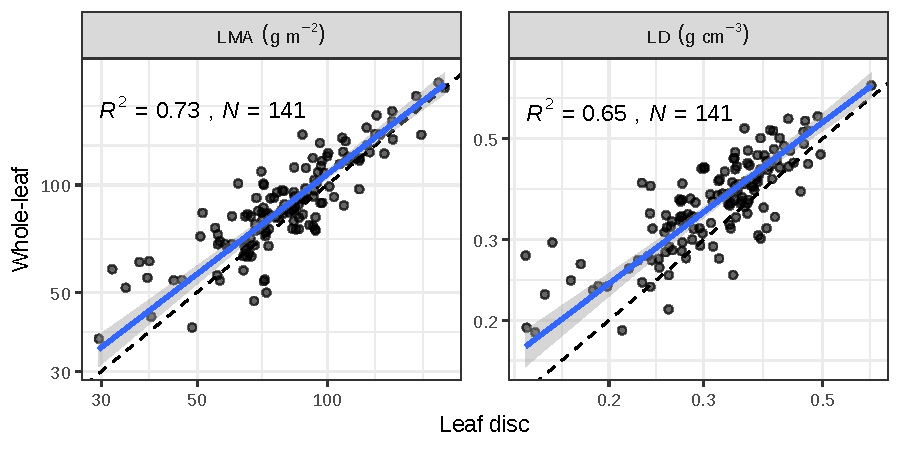
\includegraphics[width=6.25in,height=\textheight]{../figs/lma_ld.pdf}

Figure: Relationships between species mean leaf mass per area (LMA) and
leaf tissue density (LD) determined by using whole leaves and leaf discs
for the Yunnan dataset that has both leaf thickness for leaf discs and
whole leaves. Dashed lines indicate 1:1 lines. Blue solid lines indicate
standardized major axis regressions. The 95\% confidence intervals are
presented as the shaded area. All the correlations are significant
(\emph{P} \textless{} 0.001).

\newpage

\hypertarget{figure-s3}{%
\section{Figure S3:}\label{figure-s3}}

Standardized regression coefficients modelig the effects of leaf tissue
density, leaf area, leaf thickness, punch size, and their interactios
(a) on the mean estimates of whole-leaf LMA, and (b) on the estimated
variance of whole-leaf LMA. The leaf disc LMA was used for the baseline
mean of the whole-leaf LMA. Thick and thin lines indicate 90\% and 95\%
credible intervals, respectively. Circles show posterior means of
coefficients. Circles filled with blue indicate significant effects and
white indicate non-significance effects.

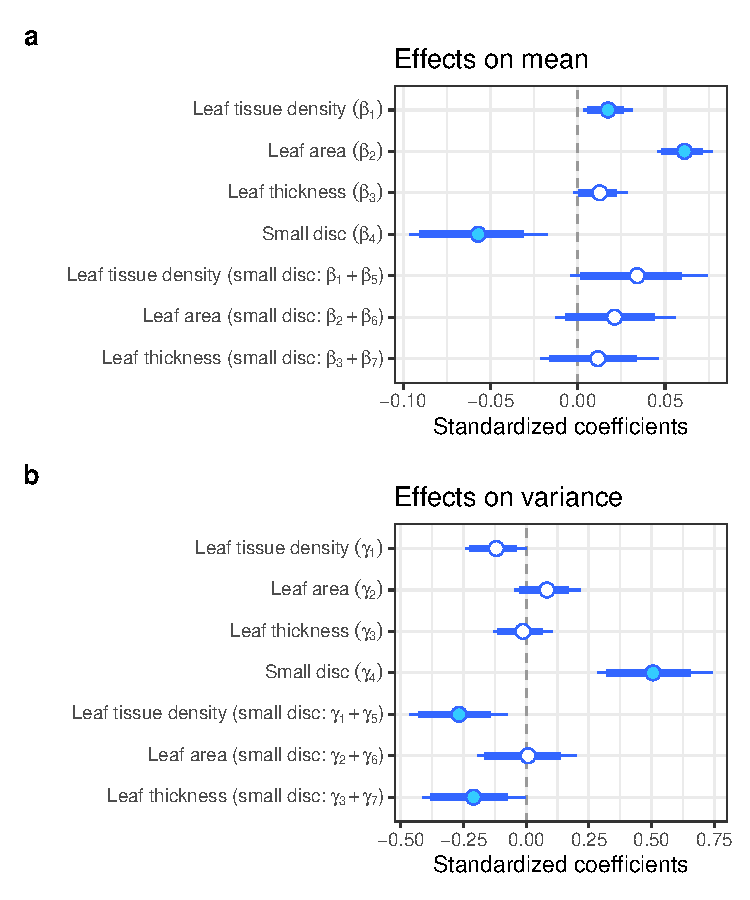
\includegraphics{../figs/coef_sp_punch1_add.pdf}

\newpage

\hypertarget{figure-s4}{%
\section{Figure S4:}\label{figure-s4}}

Relationships between species mean leaf mass per area (LMA) determined
by using whole-leaves and leaf discs for species obtained with leaf
punches of different diameters. Dashed lines indicate 1:1 lines. Blue
solid lines indicate standardized major axis (SMA) regressions. The 95\%
confidence intervals are resented as the shaded area. The correlation is
significant (\emph{P} \textless{} 0.001).

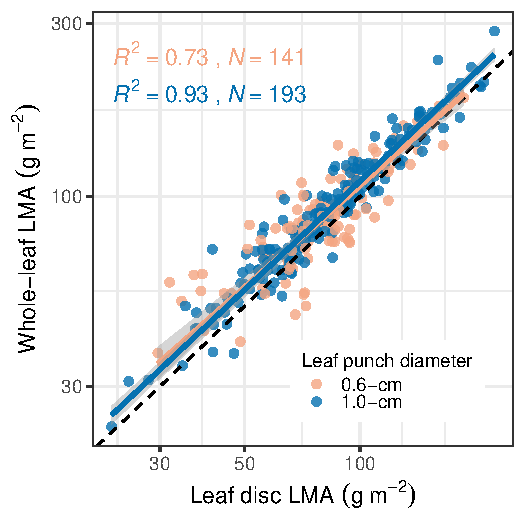
\includegraphics[width=4.16667in,height=\textheight]{../figs/sma_sep.pdf}

\newpage

\hypertarget{figure-s5}{%
\section{Figure S5:}\label{figure-s5}}

Relationships between whole-leaf LMA : disc leaf LMA and total dry mass
for the leaf disc. The relationships was heteroscedastic (unequal
variance, \emph{p} \textless{} 0.001; all the samples were analyzed
together). Samples with small total dry mass tended to show greater
variance.

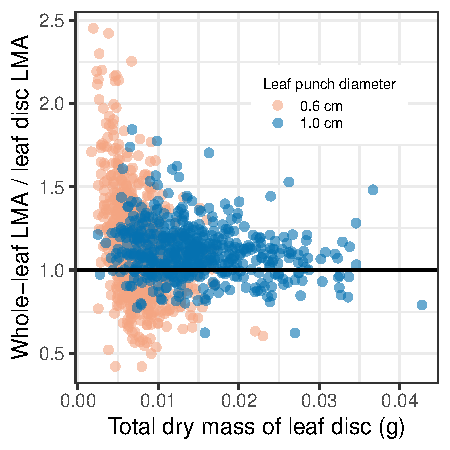
\includegraphics[width=4.16667in,height=\textheight]{../figs/ratio_dm.pdf}

\newpage

\hypertarget{literature-cited}{%
\section*{LITERATURE CITED}\label{literature-cited}}
\addcontentsline{toc}{section}{LITERATURE CITED}

\hypertarget{refs}{}
\begin{CSLReferences}{1}{0}
\leavevmode\vadjust pre{\hypertarget{ref-Eguchi2006}{}}%
Eguchi, T. 2006. Climate. Yakushima, 3--26. {Asakura Shoten}, {Tokyo (in
Japanese)}.

\leavevmode\vadjust pre{\hypertarget{ref-Fei2018}{}}%
Fei, X., Q. Song, Y. Zhang, Y. Liu, L. Sha, G. Yu, L. Zhang, et al.
2018. \href{https://doi.org/10.1016/j.scitotenv.2017.10.239}{Carbon
exchanges and their responses to temperature and precipitation in forest
ecosystems in {Yunnan}, {Southwest China}}. \emph{Science of The Total
Environment} 616--617: 824--840.

\leavevmode\vadjust pre{\hypertarget{ref-Song2017}{}}%
Song, Q. H., Y. P. Zhang, L. Q. Sha, X. B. Deng, Y. Deng, C. S. Wu, Z.
Y. Lu, et al. 2017. \href{https://doi.org/10.3832/ifor2223-010}{Canopy
temperature variability in a tropical rainforest, subtropical evergreen
forest, and savanna forest in {Southwest China}}. \emph{iForest -
Biogeosciences and Forestry} 10: 611.

\end{CSLReferences}

\end{document}
